\section{Herramienta 2: Error relativo}

\begin{frame}{¿Qué es el error relativo?}
  \begin{block}{Definición}
    Mide qué tan lejos está el resultado real del resultado ideal, en porcentaje:
    \[
      E_r = \frac{|F_{opt} - F_{real}|}{F_{opt}} \times 100\%
    \]
  \end{block}
  \vspace{0.5em}
  \begin{itemize}
    \item \(F_{opt}\): oro que \textit{deberías} tener si farmearas perfecto (nivel Inmortal).
    \item \(F_{real}\): oro que \textit{realmente} tienes (nivel Promedio).
  \end{itemize}
\end{frame}

\begin{frame}{Ejemplo numérico}
  \begin{itemize}
    \item Cálculo teórico al minuto 10: \(F_{opt} = 5600\) oro (Luna Inmortal).
    \item Resultado real en partida: \(F_{real} = 3700\) oro (Luna Promedio).
  \end{itemize}
  \vspace{0.5em}
  \[
    E_r = \frac{|5600 - 3700|}{5600} \times 100\% = 33.9\%
  \]
  \vspace{0.5em}
  \begin{block}{Interpretación}
    \begin{itemize}
      \item \(0\%\): farmeo perfecto.
      \item \(33.9\%\): se perdió un tercio del oro posible.
      \item El objetivo del proyecto es \textbf{reducir ese porcentaje}.
    \end{itemize}
  \end{block}
\end{frame}

\begin{frame}{Curvas de Farmeo: Óptimo (Inmortal) vs Promedio}
  \begin{center}
    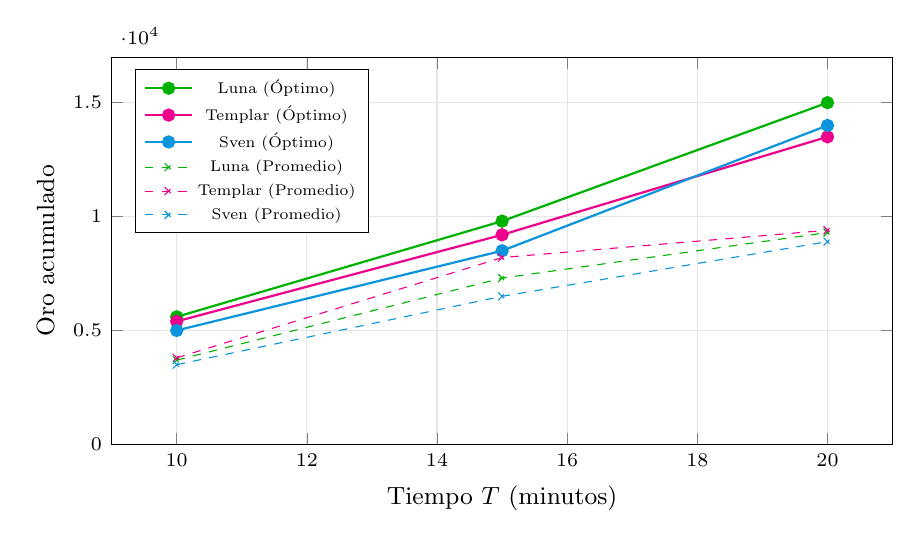
\begin{tikzpicture}
      \begin{axis}[
        width=11.5cm, height=6.5cm,
        xlabel={Tiempo \(T\) (minutos)},
        ylabel={Oro acumulado},
        xmin=9, xmax=21, ymin=0, ymax=17000,
        grid=major, grid style={gray!20},
        legend pos=north west,
        legend style={font=\scriptsize, nodes={scale=0.8, transform shape}},
        tick label style={font=\scriptsize},
        label style={font=\small},
      ]
        % Datos Óptimos (Inmortales) - Líneas Sólidas
        \addplot[green!70!black, thick, mark=*, domain=10:20] 
          coordinates {(10,5600) (15,9800) (20,15000)};
        \addlegendentry{Luna (Óptimo)}
        
        \addplot[magenta, thick, mark=*, domain=10:20] 
          coordinates {(10,5400) (15,9200) (20,13500)};
        \addlegendentry{Templar (Óptimo)}
        
        \addplot[cyan!80!blue, thick, mark=*, domain=10:20] 
          coordinates {(10,5000) (15,8500) (20,14000)};
        \addlegendentry{Sven (Óptimo)}

        % Datos Promedio (Medallas bajas) - Líneas Punteadas
        \addplot[green!70!black, dashed, mark=x, domain=10:20] 
          coordinates {(10,3700) (15,7300) (20,9300)};
        \addlegendentry{Luna (Promedio)}
        
        \addplot[magenta, dashed, mark=x, domain=10:20] 
          coordinates {(10,3800) (15,8200) (20,9400)};
        \addlegendentry{Templar (Promedio)}
        
        \addplot[cyan!80!blue, dashed, mark=x, domain=10:20] 
          coordinates {(10,3500) (15,6500) (20,8900)};
        \addlegendentry{Sven (Promedio)}
      \end{axis}
    \end{tikzpicture}
  \end{center}
  \vspace{-0.2em}
  \begin{center}
    \scriptsize La brecha entre las líneas sólidas y punteadas representa el oro perdido por falta de optimización en las rutas.
  \end{center}
\end{frame}

\begin{frame}{Error relativo a lo largo de la partida}
  \begin{center}
    \begin{tikzpicture}
      \begin{axis}[
        width=11cm, height=6cm,
        xlabel={Tiempo \(T\) (minutos)},
        ylabel={\(E_r\) (\%)},
        xmin=0, xmax=20, ymin=0, ymax=45,
        grid=major, grid style={gray!20},
        tick label style={font=\scriptsize},
        label style={font=\small},
      ]
        % Curva de error simulada (basada en la brecha de los datos reales)
        \addplot[realcolor, thick, mark=*, mark size=1.5pt] coordinates {
          (10,33) (15,25) (20,38)
        };
        \addplot[gray, dashed, domain=0:20] {30};
        \node[font=\scriptsize, gray] at (axis cs:12,32) {umbral crítico};
      \end{axis}
    \end{tikzpicture}
  \end{center}
  \vspace{-0.3em}
  \begin{center}
    \small El error fluctúa según el héroe, pero tiende a mantenerse alto si no se optimizan las rutas.
  \end{center}
\end{frame}